% Manuscript draft for Socio-Economic Planning Sciences.
% Uses elsarticle when available (Overleaf has it); otherwise falls back to article for local previews.
\IfFileExists{elsarticle.cls}{%
  \documentclass[preprint,12pt,number]{elsarticle}%
  \def\ELSAVAILABLE{1}%
}{%
  \documentclass[11pt,a4paper]{article}%
  \usepackage[margin=2.5cm]{geometry}%
  \usepackage[numbers,sort&compress]{natbib}%
  \newenvironment{frontmatter}{}{}%
  \newenvironment{keyword}{\par\noindent\textbf{Keywords:} }{\par}%
  \newcommand{\address}[2][]{}%
  \newcommand{\journal}[1]{}%
  \newcommand{\sep}{; }%
}
\usepackage{amsmath,amssymb,amsthm,mathtools}
\usepackage{booktabs,graphicx,xcolor,array}
\usepackage{algorithm,algpseudocode}
\usepackage[hidelinks]{hyperref}
\usepackage{cleveref}

\newtheorem{theorem}{Theorem}
\newtheorem{proposition}{Proposition}
\newtheorem{corollary}{Corollary}
\newtheorem{lemma}{Lemma}
\theoremstyle{definition}
\newtheorem{definition}{Definition}
\newtheorem{assumption}{Assumption}
\theoremstyle{remark}
\newtheorem{remark}{Remark}

\newcommand{\R}{\mathbb{R}}
\newcommand{\U}{\mathcal{U}}
\newcommand{\I}{\mathcal{I}}
\newcommand{\pimax}{\pi^{\max}}
\newcommand{\todo}[1]{\textcolor{red}{[TODO: #1]}}
\newcommand{\prelim}[1]{\textcolor{blue}{#1}}

\journal{Socio-Economic Planning Sciences}

\begin{document}

\begin{frontmatter}

\title{A conformally calibrated linear-fractional robust model for food-indexed cash transfers and price monitoring under partial information}

\author{Maniru Ibrahim\todo{co-authors and affiliations}}
\address{University of Limerick, Limerick, Ireland}
\ifdefined\ELSAVAILABLE\else\maketitle\fi

\begin{abstract}
Food-indexed cash transfers keep their value only if payments follow local food prices, but planners rarely observe those prices directly. They see national or zonal averages, the highest- and lowest-priced states and delayed surveys. We study how to allocate a fixed transfer budget across regions under this partial information. The protection a rule gives every recipient is the product of budget adequacy and allocative efficiency. Over any polytope of admissible prices, the allocation that maximises worst-case efficiency pays each region in proportion to its largest possible need share, and each share is a linear-fractional program that reduces to a linear program. For polytopes built from group averages the shares follow from sorting and a Dinkelbach iteration, for boxes on regional needs they have a closed form, and a water-filling rule trades expected performance against the worst case. The uncertainty set is calibrated by conformal prediction, so the guarantee holds with a stated probability. The same guarantee is used to decide which regions to monitor. The model is applied to Nigeria with 125,598 state--item--month food prices from January 2017 to August 2023 and food budgets of poor households from the 2018/19 living standards survey. A flat transfer delivered on average 82\% of the protection the same budget could buy and 70\% in the worst month, and indexing to zonal averages did worse than the flat rule in 34 of 54 months. Over 2021 to 2023 a guarantee-constrained rule realised 91\% against 78\% for the flat rule and certified 64\% in the worst case against 40\%. The certificates held in every month, and the calibrated sets covered true needs in 87\% of months at an 80\% target. Monitoring five states without delay raised the guarantee from 0.72 to 0.79, while a one-month reporting delay removed most of this gain. Between September 2023 and May 2026, when no state food prices were published, the guarantee fell from 0.88 to 0.67 and the certificate of the flat rule from 0.70 to 0.39.
\end{abstract}

\begin{keyword}
Robust optimization \sep Linear-fractional programming \sep Conformal prediction \sep Cash transfers \sep Food price monitoring \sep Nigeria
\end{keyword}

\end{frontmatter}

% =====================================================================
\section{Introduction}\label{sec:intro}

Nigeria removed its petrol subsidy in May 2023 and unified its exchange-rate windows in June 2023 \citep{tinubu2023inaugural,cbn2023fx}. Food prices rose sharply in the following months, and they had already diverged across states before the reforms. In the state food price data of the National Bureau of Statistics (NBS), the cost of a poor household's food basket grew twice as fast in the most exposed state as in the least exposed state between January 2019 and mid-2021 (\cref{sec:case}). The federal response included a cash transfer to 15 million households, launched in October 2023, of N75,000 per household paid in three instalments and financed in part by an \$800 million World Bank operation \citep{nairametrics2023nassp}. The amount was the same in every state.

When local prices diverge, a uniform payment buys less food where prices have risen most. Indexing payments to local prices would correct this, but it requires local prices that the planner usually does not have. The NBS published its last complete table of state food prices for August 2023, and no table exists for June 2023. Since September 2023 it has released national and zonal averages and, for each item, the names and prices of the most and least expensive states \citep{nbs2026econs}. Some compiled datasets fill the missing months by copying each zonal average to every state of the zone, which removes the variation that indexation needs. A planner who wants to index payments therefore has to decide with aggregates, extremes and old state data, and has to decide whether better data are worth collecting.

\subsection{Research questions}\label{sec:rq}

This study addresses three research questions.

(Q1) How should a fixed transfer budget be allocated across states when local prices are observed only through aggregates, extremes and delayed observations? We measure the protection of a rule by the share of a food entitlement that every recipient can buy, and we look for the allocation that keeps this share as high as possible for all prices consistent with the available information. The problem has a ratio objective, and we show that it has a closed-form solution.

(Q2) How much protection can such an allocation guarantee, and how can the guarantee be made statistically valid? A worst-case guarantee is only as reliable as the uncertainty set behind it. Instead of fixing the set by assumption, we calibrate it by conformal prediction so that it contains the true prices or needs with a stated probability, and we adapt the calibration when the price process shifts and when state data stop arriving.

(Q3) Which states should a monitoring system observe, and how quickly, to raise the guarantee most? Collecting state prices is costly. We choose the monitored states by the guarantee of the allocation that uses them, and we compare this choice with one based on forecast accuracy and with monitoring that reports late.

\subsection{Contributions of our work}\label{sec:contrib}

The contributions of this work are as follows.

(i) Model. We formulate the allocation of a transfer budget across regions as an equal-protection problem in which needs are linear in uncertain prices. For known prices, the protection of any rule is the product of budget adequacy and allocative efficiency (\cref{prop:fullinfo}). The first term depends only on the size of the budget and the second only on its distribution, so the two can be analysed separately.

(ii) Robust solution and its computation. Over any polytope of admissible prices, the allocation with the best worst-case efficiency pays each region in proportion to its largest possible need share, and its guarantee is the reciprocal of the recipient-weighted sum of these shares (\cref{thm:robust}). Each share is a linear-fractional program, solved as a linear program by the transformation of \citet{charnes1962programming} (\cref{prop:cc}). For polytopes built from group averages, which describe what statistical agencies publish, the shares follow from sorting and a Dinkelbach iteration (\cref{prop:knapsack}). For boxes on regional needs they have a closed form (\cref{prop:needbox}). A water-filling rule gives the allocation with the best expected performance among those that keep a chosen fraction of the guarantee (\cref{prop:kappa}).

(iii) Calibrated guarantee. The uncertainty set is calibrated by split and adaptive conformal prediction \citep{vovk2005algorithmic,gibbs2021aci}, which gives the guarantee a coverage probability (\cref{prop:conformal}). For periods without state data, the sets are calibrated by forecast horizon and widened monotonically, so the guarantee declines as information ages.

(iv) Monitoring design and evidence. The expected guarantee is monotone in the set of monitored regions (\cref{prop:monotone}) and is used to select them. On 125,598 genuine state--item--month prices from Nigeria, monitoring chosen this way gives higher guarantees than monitoring chosen for forecast accuracy, and reporting delay limits the gain more than the number of monitored states does. We also apply the model to September 2023 to May 2026, when only aggregates and state extremes were published.

The rest of the paper is organised as follows. \Cref{sec:lit} reviews related work. \Cref{sec:model} describes the problem and the model. \Cref{sec:robust} derives the robust allocation and its guarantee. \Cref{sec:conformal} calibrates the uncertainty set, and \cref{sec:monitor} treats monitoring design. \Cref{sec:case} presents the Nigerian case study. \Cref{sec:discussion} discusses implications for programmes and statistical agencies, and \cref{sec:conclusion} concludes.

% =====================================================================
\section{Literature review}\label{sec:lit}

This section reviews the studies related to our problem. The first part covers the allocation of cash transfers and food assistance. The second covers spatial price differences and the measurement of local prices. The third covers the methods used to handle uncertainty in such models, including conformal prediction and the choice of what data to collect. The last part identifies the gaps and explains how our work addresses them.

\subsection{Allocation of cash transfers and food assistance}

Research on cash transfers has concentrated on targeting, that is, on deciding who receives a payment when household welfare is observed with error. \citet{hanna2018ubi} compare universal and targeted transfers in developing countries and discuss the costs of imperfect targeting. \citet{aiken2022phone} use mobile phone data and machine learning to target humanitarian aid in Togo. \citet{zheng2022targeting} go from targeting to the size of the transfer: they compare predictive, stochastic and robust allocation rules that minimise the squared shortfall from the poverty line when targeting errors are known in distribution, and they show that a predictive rule is optimal when these errors are well calibrated. In an experiment in northern Ecuador, cash, food and vouchers all raised food consumption, while their costs and their effects on the composition of diets differed \citep{hidrobo2014cash}. In humanitarian practice, transfer values follow the cost of a minimum expenditure basket. Revisions are triggered when cumulative price changes exceed a threshold, and separate values by area are recommended when local prices depart from national trends \citep{gfsc2023inflation}.

In operations research, food assistance has mostly been studied as a distribution problem. \citet{orgut2016modeling} allocate donated food across counties served by a food bank so as to limit deviations from a proportional share, with a sensitivity analysis on receiving capacities. \citet{eisenhandler2019humanitarian} combine routing and allocation in daily food rescue operations with an objective that balances quantity and equity. \citet{dawood2026fima} build a machine-learning food insecurity index and feed it into an equitable allocation model for a South African food bank. On the network side, \citet{rancourt2015tactical} locate food aid distribution centres in Kenya, and \citet{noyan2016stochastic} design last-mile relief networks under demand and network uncertainty by two-stage stochastic programming. \citet{demoor2024robust} develop robust and adaptive robust models for food aid procurement when purchase prices are uncertain. In these studies the recipients or demand points are uncertain or the logistics are the decision. None of them allocates a cash budget when the uncertainty is in the local prices that recipients pay.

\subsection{Spatial price differences and local price information}

Prices differ across the regions of large countries, and welfare comparisons that ignore these differences misrank households and places \citep{deaton1997analysis,deaton2011spatial}. The effect is largest for the poor, whose budgets are dominated by food, and in many low-income countries the consumer price index is compiled from a small number of urban markets. \citet{dietrich2023lost} compare national price indices with local market prices in seven West African countries and find that using local prices changes who is classified as food poor, with inclusion and exclusion errors of about 5\% and 2\%. They argue for systematic collection of local prices to support transfers indexed to prices. When local surveys are incomplete, \citet{andree2021estimating} recovers market-level food price inflation by machine-learning imputation for 25 fragile countries. These studies measure the cost of missing local price information for poverty statistics. They do not ask how a budget should be allocated when that information is incomplete, or how much a given set of observations is worth to that allocation.

\subsection{Uncertainty modelling and data collection}

Stochastic programming (SO), robust optimisation (RO) and distributionally robust optimisation (DRO) are the main approaches to parameter uncertainty in allocation models. SO needs a probability distribution of the parameters, as in the relief network model of \citet{noyan2016stochastic}. RO protects a decision against every realisation in an uncertainty set \citep{bental2009robust}, and the conservatism of the solution depends on the size of the set \citep{bertsimas2004price}. \citet{bertsimas2018datadriven} construct uncertainty sets from data with statistical guarantees, and \citet{esfahani2018datadriven} give finite-sample guarantees for DRO over Wasserstein balls. Robust and distributionally robust models are increasingly used in socio-economic planning, for example for the location and pricing of agricultural machinery services under demand uncertainty \citep{zhang2026robust}. Predictive and prescriptive analytics connect forecasts with decisions \citep{bertsimas2020predictive,elmachtoub2022spo}. Our objective is a ratio, which places the problem in linear-fractional programming \citep{charnes1962programming,dinkelbach1967nonlinear,schaible1983fractional}.

Conformal prediction gives finite-sample coverage under exchangeability without distributional assumptions \citep{vovk2005algorithmic,romano2019cqr}. Adaptive conformal inference controls the long-run miss rate under distribution shift \citep{gibbs2021aci}, and \citet{barber2023beyond} bound the loss of coverage when exchangeability fails. Several recent studies use conformal sets as uncertainty sets in robust optimisation. \citet{johnstone2021conformal} calibrate ellipsoidal and box sets, \citet{sun2023predict} calibrate the uncertainty of a fixed predictor for robust contextual linear programs, \citet{patel2024conformal} build conformal regions from generative models, and \citet{chenreddy2024endtoend} and \citet{yeh2025endtoend} train the uncertainty set together with the decision. These methods are general. They do not use the structure of an allocation problem, and they do not consider which data should be collected.

The choice of what to observe has been studied as a value-of-information problem \citep{howard1966information} and, in spatial settings, as sensor placement, where locations are chosen by greedy algorithms that maximise an information criterion with guarantees for submodular objectives \citep{nemhauser1978analysis,minoux1978accelerated,krause2008near}. In these models the criterion is statistical, such as entropy or mutual information, and is not tied to a downstream decision.

\subsection{Distinction of our work from the existing literature}

\Cref{tab:positioning} classifies the related studies by decision, uncertainty, modelling approach, guarantee, data collection and solution method. Our work differs from the existing literature in four respects. First, previous allocation models treat the recipients, their welfare or the logistics as uncertain \citep{zheng2022targeting,orgut2016modeling,noyan2016stochastic}, while we allocate a cash budget when the uncertainty is in the local prices that recipients pay, and we model the information that agencies actually publish as linear constraints. Second, the robust allocation has a closed form, and the worst-case shares are computed exactly by linear programming, by sorting with a Dinkelbach iteration, or in closed form, depending on the information available. Third, the uncertainty set is calibrated by conformal prediction, which gives the guarantee a stated coverage probability; in contrast to the general conformal robust optimisation methods \citep{johnstone2021conformal,patel2024conformal,yeh2025endtoend}, the calibration is tied to a single scalar guarantee and extended to information that becomes stale. Fourth, we use the same guarantee to choose which regions to monitor and to compare monitoring with and without reporting delay, which links the measurement literature \citep{dietrich2023lost,andree2021estimating} to the allocation decision.

\begin{table}[t]
\centering
\caption{Related literature and positioning of this paper.}\label{tab:positioning}
\footnotesize
\setlength{\tabcolsep}{3.5pt}
\begin{tabular}{lcccccccl}
\toprule
Reference & \rotatebox{90}{Allocation} & \rotatebox{90}{Local prices} & \rotatebox{90}{Uncertainty} & \rotatebox{90}{Type of uncertainty} & \rotatebox{90}{Methodology} & \rotatebox{90}{Guarantee} & \rotatebox{90}{Data collection} & \rotatebox{90}{Solution approach}\\
\midrule
\citet{hanna2018ubi} & \checkmark & -- & -- & -- & EA & -- & -- & --\\
\citet{hidrobo2014cash} & \checkmark & -- & -- & -- & RCT & -- & -- & --\\
\citet{aiken2022phone} & \checkmark & -- & \checkmark & Welfare & ML & -- & -- & ML\\
\citet{zheng2022targeting} & \checkmark & -- & \checkmark & Welfare & SO, RO & -- & -- & CF, OCO\\
\citet{orgut2016modeling} & \checkmark & -- & \checkmark & Capacity & SA & -- & -- & OPT.SOL\\
\citet{eisenhandler2019humanitarian} & \checkmark & -- & -- & -- & -- & -- & -- & Exact, LNS\\
\citet{dawood2026fima} & \checkmark & -- & -- & -- & ML & -- & -- & OPT.SOL\\
\citet{rancourt2015tactical} & \checkmark & -- & -- & -- & -- & -- & -- & OPT.SOL\\
\citet{noyan2016stochastic} & \checkmark & -- & \checkmark & Demand, network & SO & -- & -- & BD\\
\citet{demoor2024robust} & \checkmark & \checkmark & \checkmark & Procurement price & RO, ARO & -- & -- & OPT.SOL\\
\citet{zhang2026robust} & -- & -- & \checkmark & Demand & GDRO & -- & -- & Bi-level alg.\\
\citet{dietrich2023lost} & -- & \checkmark & -- & -- & EA & -- & -- & --\\
\citet{andree2021estimating} & -- & \checkmark & \checkmark & Missing prices & ML & -- & -- & ML\\
\citet{bertsimas2018datadriven} & -- & -- & \checkmark & Generic & RO & \checkmark & -- & OPT.SOL\\
\citet{esfahani2018datadriven} & -- & -- & \checkmark & Distribution & DRO & \checkmark & -- & CR\\
\citet{johnstone2021conformal} & -- & -- & \checkmark & Generic & CP, RO & \checkmark & -- & OPT.SOL\\
\citet{sun2023predict} & -- & -- & \checkmark & Cost vector & CP, RO & \checkmark & -- & OPT.SOL\\
\citet{patel2024conformal} & -- & -- & \checkmark & Generic & CP, RO & \checkmark & -- & GD\\
\citet{chenreddy2024endtoend} & -- & -- & \checkmark & Generic & RO & -- & -- & GD\\
\citet{yeh2025endtoend} & -- & -- & \checkmark & Generic & CP, RO & \checkmark & -- & GD\\
\citet{krause2008near} & -- & -- & \checkmark & Spatial field & GP & -- & \checkmark & Greedy\\
This paper & \checkmark & \checkmark & \checkmark & Prices, needs & CP, RO & \checkmark & \checkmark & CF, DK, Greedy\\
\bottomrule
\end{tabular}

\vspace{2pt}
\parbox{\textwidth}{\scriptsize EA: empirical analysis. RCT: randomised controlled trial. ML: machine learning. SO: stochastic optimisation. RO: robust optimisation. ARO: adaptive robust optimisation. DRO: distributionally robust optimisation. GDRO: globalized DRO. SA: sensitivity analysis. CP: conformal prediction. GP: Gaussian process. CF: closed form. OCO: online convex optimisation. LNS: large neighbourhood search. BD: Benders decomposition. CR: convex reformulation. GD: gradient-based training. DK: Dinkelbach iteration. OPT.SOL: optimisation solver. ``--'': not considered.}
\end{table}

% =====================================================================
\section{Problem description and model}\label{sec:model}

\subsection{Setting and notation}

Let $S$ be the set of states ($|S|=37$, including the Federal Capital Territory) and $J$ a reference basket of food items. In month $t$, $p_{sjt}>0$ is the average retail price of item $j$ in state $s$, and $p_t\in\R^{S\times J}_{+}$ stacks these prices. A programme with $N_s>0$ recipients in state $s$ promises each recipient a food entitlement worth $T_0$ in a base month $0$, where the base basket has quantities $q_j\ge 0$ and costs $C_{s0}=\sum_j q_j p_{sj0}$ in state $s$. Keeping that entitlement intact in month $t$ requires
\begin{equation}\label{eq:need}
D_{s}(p_t) \;=\; T_0\,\frac{\sum_j q_j\,p_{sjt}}{C_{s0}} \;=\; a_s^{\top}p_t,
\qquad a_{sj}=\frac{T_0\,q_j}{C_{s0}}\ \text{on the block of state } s,
\end{equation}
so need is linear in prices. We drop the subscript $t$ when no confusion arises. The planner has a budget $B>0$ and chooses payments $T=(T_s)_{s\in S}$ in the feasible set
\begin{equation}\label{eq:feasible}
\mathcal{T}(B)=\Big\{T\in\R^{S}_{+}:\ \textstyle\sum_{s}N_sT_s=B\Big\}.
\end{equation}

\subsection{Protection, adequacy and efficiency}

\begin{definition}[Protection]
The protection delivered by $T$ at prices $p$ is the share of the entitlement guaranteed to every recipient,
\begin{equation}\label{eq:protection}
\rho(T,p)=\min_{s\in S}\frac{T_s}{D_s(p)}.
\end{equation}
\end{definition}

\begin{proposition}[Full information]\label{prop:fullinfo}
For known prices $p$, $\max_{T\in\mathcal T(B)}\rho(T,p)=\rho^*(p)=B/\sum_{k}N_kD_k(p)$, attained uniquely by $T_s=\rho^*(p)\,D_s(p)$. Consequently, for every $T\in\mathcal T(B)$,
\begin{equation}\label{eq:decomp}
\rho(T,p)=\rho^*(p)\times E(T,p),\qquad E(T,p)=\frac{\rho(T,p)}{\rho^*(p)}\in(0,1],
\end{equation}
where $\rho^*(p)$ depends only on the budget (\emph{adequacy}) and $E(T,p)$ is invariant to rescaling the budget (\emph{allocative efficiency}).
\end{proposition}

\begin{proof}
Let $T\in\mathcal T(B)$ and $\rho=\rho(T,p)$. Then $T_s\ge\rho D_s(p)$ for all $s$, so $B=\sum_sN_sT_s\ge\rho\sum_sN_sD_s(p)$, that is $\rho\le\rho^*(p)$. The allocation $T_s=\rho^*(p)D_s(p)$ is feasible and attains the bound. If $T$ attains the bound, every inequality $T_s\ge\rho^*D_s$ must hold with equality because $N_s>0$, which gives uniqueness. Finally, if $T$ is replaced by $cT$ and $B$ by $cB$ for $c>0$, both $\rho(T,p)$ and $\rho^*(p)$ scale by $c$, so $E$ is unchanged.
\end{proof}

A budget that is too small lowers adequacy for every recipient, and a budget spent in the wrong places lowers efficiency. For the uniform rule $T_s\equiv B/\sum_kN_k$,
\begin{equation}\label{eq:flat}
E_{\mathrm{flat}}(p)=\frac{\sum_kN_kD_k(p)\big/\sum_kN_k}{\max_sD_s(p)},
\end{equation}
the recipient-weighted mean need divided by the largest need.

\subsection{Partial information as a price polytope}

At decision time the planner holds an information set $\I_t$, which we translate into a set $\U_t\subset\R^{S\times J}_{+}$ of price vectors consistent with it. All information used here gives linear constraints:
\begin{itemize}
\item[(U1)] \emph{monitored prices}: $p_{sjt}=o_{sjt}$ for $(s,j)$ in a monitored set $M$;
\item[(U2)] \emph{published national averages} $A_{jt}$: $(1-\varepsilon)A_{jt}\le|S|^{-1}\sum_sp_{sjt}\le(1+\varepsilon)A_{jt}$;
\item[(U3)] \emph{published zonal averages}: the same constraint for each geopolitical zone;
\item[(U4)] \emph{published extremes} $H_{jt}$ and $L_{jt}$ attained in named states $h$ and $l$: $p_{hjt}=H_{jt}$, $p_{ljt}=L_{jt}$ and $L_{jt}\le p_{sjt}\le H_{jt}$ for all $s$;
\item[(U5)] \emph{calibrated relative-price bands}: $\ell_{sjt}A_{jt}\le p_{sjt}\le u_{sjt}A_{jt}$ (\cref{sec:conformal});
\item[(U6)] \emph{delayed observations} from $d$ months earlier: $g^{\ell}_{sjt}\,p_{sj,t-d}\le p_{sjt}\le g^{u}_{sjt}\,p_{sj,t-d}$.
\end{itemize}

\begin{assumption}\label{ass:polytope}
$\U_t$ is a nonempty bounded polytope, $\U_t=\{p\ge 0:\ \underline p\le p\le\overline p,\ Rp\le r\}$, and $D_s(p)>0$ for all $s$ and $p\in\U_t$.
\end{assumption}

The audit in \cref{sec:case} calibrates $\varepsilon$: published national averages equal the unweighted mean of state prices in 78\% of item--months, and the tolerance is set from the distribution of the remaining gaps.

% =====================================================================
\section{Robust allocation and its guarantee}\label{sec:robust}

Define the \emph{need share} of state $s$ and its worst case over $\U$:
\begin{equation}\label{eq:share}
\pi_s(p)=\frac{D_s(p)}{\sum_kN_kD_k(p)},\qquad
\pimax_s(\U)=\max_{p\in\U}\pi_s(p).
\end{equation}
Note that $\sum_sN_s\pi_s(p)=1$ for every $p$, and the maximum in \eqref{eq:share} exists because $\pi_s$ is continuous on the compact set $\U$.

\begin{theorem}[Closed-form robust allocation]\label{thm:robust}
Under \cref{ass:polytope},
\begin{equation}\label{eq:maximin}
\max_{T\in\mathcal T(B)}\ \min_{p\in\U}\ E(T,p)\;=\;G(\U)\;=\;\frac{1}{\sum_{s}N_s\,\pimax_s(\U)},
\end{equation}
and the maximum is attained uniquely by
\begin{equation}\label{eq:Trob}
T^{\mathrm{rob}}_s=B\,\frac{\pimax_s(\U)}{\sum_kN_k\,\pimax_k(\U)},\qquad s\in S.
\end{equation}
Moreover $0<G(\U)\le 1$, with $G(\U)=1$ when $\U$ is a single point.
\end{theorem}

\begin{proof}
Fix $T\in\mathcal T(B)$. By \cref{prop:fullinfo},
\[
E(T,p)=\frac{\min_s T_s/D_s(p)}{B/\sum_kN_kD_k(p)}=\min_{s\in S}\frac{T_s}{B\,\pi_s(p)}.
\]
Minimising over $p\in\U$ and exchanging the two minimisations gives
\[
\min_{p\in\U}E(T,p)=\min_{s\in S}\ \min_{p\in\U}\frac{T_s}{B\,\pi_s(p)}=\min_{s\in S}\frac{T_s}{B\,\pimax_s(\U)}=:\theta(T).
\]
Since $T_s\ge\theta(T)\,B\,\pimax_s$ for all $s$, the budget gives $B=\sum_sN_sT_s\ge\theta(T)\,B\sum_sN_s\pimax_s$, so $\theta(T)\le G(\U)$. The allocation \eqref{eq:Trob} is feasible and has $T_s/(B\pimax_s)=G(\U)$ for every $s$, so it attains the bound. If $\theta(T)=G(\U)$, every inequality $T_s\ge G\,B\,\pimax_s$ holds with equality because $N_s>0$, which proves uniqueness. For any $p_0\in\U$, $\sum_sN_s\pimax_s\ge\sum_sN_s\pi_s(p_0)=1$, so $G\le 1$; if $\U=\{p_0\}$ the inequality is an equality.
\end{proof}

\begin{corollary}[Monotonicity]\label{cor:mono}
If $\U'\subseteq\U$ then $\pimax_s(\U')\le\pimax_s(\U)$ for all $s$ and hence $G(\U')\ge G(\U)$. Additional information never lowers the guarantee.
\end{corollary}

\begin{remark}
The guarantee in \eqref{eq:maximin} is a competitive ratio: whatever prices materialise in $\U$, $T^{\mathrm{rob}}$ delivers at least a fraction $G(\U)$ of the protection that a planner with full information could deliver with the same budget. The adversarial prices differ by state: state $s$ is protected against the price vector that maximises its own need share.
\end{remark}

\begin{proposition}[Computation by linear programming]\label{prop:cc}
Under \cref{ass:polytope}, for each $s$,
\begin{equation}\label{eq:cc}
\pimax_s(\U)=\max_{y\ge0,\ \tau\ge0}\Big\{a_s^{\top}y:\ Ry\le r\tau,\ \underline p\,\tau\le y\le\overline p\,\tau,\ \textstyle\sum_kN_k\,a_k^{\top}y=1\Big\},
\end{equation}
and an optimal $p$ in \eqref{eq:share} is recovered as $y^*/\tau^*$.
\end{proposition}

\begin{proof}
Write $d(p)=\sum_kN_ka_k^{\top}p>0$ on $\U$. For $p\in\U$, the pair $(y,\tau)=(p/d(p),1/d(p))$ is feasible in \eqref{eq:cc} with objective $\pi_s(p)$, so the optimal value of \eqref{eq:cc} is at least $\pimax_s$. Conversely, let $(y,\tau)$ be feasible. If $\tau=0$, then $Ry\le0$ and $0\le y\le 0$, so $y=0$, which contradicts $\sum_kN_ka_k^{\top}y=1$. Hence $\tau>0$, $p=y/\tau\in\U$, $d(p)=1/\tau$, and $a_s^{\top}y=\pi_s(p)\le\pimax_s$. The two values are equal and the maximiser maps as stated.
\end{proof}

Computing the robust allocation therefore requires $|S|=37$ linear programs per month and information scenario (\cref{alg:robust}).

\begin{algorithm}[t]
\caption{Robust allocation in month $t$}\label{alg:robust}
\begin{algorithmic}[1]
\Require information set $\I_t$; calibrated bands; recipients $N$; budget $B$
\State Build $\U_t=\{p:\underline p\le p\le\overline p,\ Rp\le r\}$ from (U1)--(U6)
\For{$s\in S$}
  \State Solve LP \eqref{eq:cc}; store $\pimax_s$ and $p^{(s)}=y^*/\tau^*$
\EndFor
\State $G_t\gets 1/\sum_sN_s\pimax_s$; \quad $T_s\gets B\,\pimax_s\,G_t$ for all $s$
\State \Return $T$, $G_t$ and the adversarial price vectors $\{p^{(s)}\}$
\end{algorithmic}
\end{algorithm}

\subsection{Two tractable uncertainty sets}\label{sec:tractable}

\Cref{prop:cc} needs a general LP solver and, with $1{,}554$ price cells, a well-scaled formulation. Two structures that arise in practice are solved faster and more accurately.

\paragraph{Grouped price polytopes.} Suppose the cells are partitioned into groups $g\in\mathcal G$ (for example, the states of one zone for one item) and
\begin{equation}\label{eq:grouped}
\U=\Big\{p:\ \underline p\le p\le\overline p,\ \ \underline r_g\le\textstyle\sum_{c\in g}p_c\le\overline r_g\ \ (g\in\mathcal G)\Big\}.
\end{equation}
This covers (U1), (U3), (U4) and (U5) together, and (U2) and (U5) together; monitored cells and published extremes become cells with $\underline p_c=\overline p_c$. Write $b=\sum_kN_ka_k$, so that $\pi_s(p)=a_s^{\top}p/b^{\top}p$.

\begin{proposition}[Exact computation for grouped polytopes]\label{prop:knapsack}
Let $\U$ be given by \eqref{eq:grouped} and nonempty, and let $F_s(\lambda)=\max_{p\in\U}(a_s-\lambda b)^{\top}p$. Then:
\begin{enumerate}
\item[(a)] $\pimax_s(\U)$ is the unique root of $F_s$, which is convex and strictly decreasing;
\item[(b)] for fixed $\lambda$, $F_s(\lambda)$ separates into one continuous knapsack per group. With $c=a_s-\lambda b$, each group is solved by starting from $p=\underline p$, raising cells in decreasing order of $c_c$ to their upper bounds until the group sum reaches $\underline r_g$ (even if $c_c<0$), and then continuing only while $c_c>0$ and the sum is below $\overline r_g$;
\item[(c)] the Dinkelbach iteration $\lambda_{k+1}=a_s^{\top}p_k/b^{\top}p_k$, with $p_k$ a maximiser of $F_s(\lambda_k)$, increases strictly until it reaches $\pimax_s(\U)$, which it does after finitely many steps.
\end{enumerate}
\end{proposition}

\begin{proof}
(a) $F_s$ is a maximum of affine functions of $\lambda$, hence convex, and each has slope $-b^{\top}p<0$ by \cref{ass:polytope}, so $F_s$ is strictly decreasing. $F_s(\lambda)\ge0$ if and only if $a_s^{\top}p\ge\lambda b^{\top}p$ for some $p\in\U$, that is, $\lambda\le\pimax_s$. (b) The constraints of \eqref{eq:grouped} couple only cells in the same group, so the maximum is the sum of the group maxima. Within a group the problem is a fractional knapsack with unit weights, a lower and an upper capacity: any feasible point can be moved, without lowering $c^{\top}p$, to the point that fills cells in decreasing order of $c_c$, by transferring mass from a cell with smaller $c$ to one with larger $c$; mass beyond $\underline r_g$ is added only where $c_c>0$. (c) This is Dinkelbach's method. Since $F_s(\lambda_k)=a_s^{\top}p_k-\lambda_kb^{\top}p_k$, $\lambda_{k+1}-\lambda_k=F_s(\lambda_k)/b^{\top}p_k>0$ while $\lambda_k<\pimax_s$. The maximiser in (b) is a vertex of $\U$, which has finitely many, and the ratios strictly increase, so no vertex repeats.
\end{proof}

Each evaluation of $F_s$ costs one sort per group, and all states can be processed in one vectorised pass. On the Nigerian panel the iteration stops after about three evaluations, runs about 600 times faster than solving \eqref{eq:cc} with HiGHS, and returns maximisers whose constraint violations are of order $10^{-12}$, while the LP solver stops $0.06\%$ short of the optimum on this badly scaled problem.

\paragraph{Need boxes.} \Cref{thm:robust} uses prices only through the need vector, so it holds for any compact set $\mathcal D$ of positive need vectors in place of $\{D(p):p\in\U\}$. When uncertainty is modelled directly on the $|S|$ needs,
\begin{equation}\label{eq:needbox}
\mathcal D=\{D:\ L_s\le D_s\le U_s,\ s\in S\},\qquad 0<L\le U,
\end{equation}
the worst-case shares have a closed form.

\begin{proposition}[Need box]\label{prop:needbox}
For \eqref{eq:needbox},
\[
\pimax_s=\frac{U_s}{N_sU_s+\sum_{k\neq s}N_kL_k},\qquad G=\Big(\sum_sN_s\pimax_s\Big)^{-1}.
\]
\end{proposition}

\begin{proof}
$\pi_s=D_s/(N_sD_s+\sum_{k\ne s}N_kD_k)$ increases in $D_s$ and decreases in each $D_k$, $k\ne s$, and the box constrains the coordinates independently.
\end{proof}

The need box replaces 1{,}554 simultaneous price bands by 37 need bands. A simultaneous band over many cells must be wide, and \cref{sec:results} shows that the price polytope then gives a weak guarantee.

\subsection{Trading nominal performance for the guarantee}\label{sec:frontier}

$T^{\mathrm{rob}}$ maximises the worst case and ignores the most likely prices. A planner with a point forecast $\hat D$ may prefer to pay in proportion to $\hat D$ and accept a weaker guarantee. Both aims enter the following problem. For $\kappa\in[0,1]$,
\begin{equation}\label{eq:kappa}
\max_{T\in\mathcal T(B)}\ \min_{s\in S}\frac{T_s}{\hat D_s}\quad\text{s.t.}\quad\theta(T)=\min_{s}\frac{T_s}{B\,\pimax_s}\ \ge\ \kappa\,G .
\end{equation}

\begin{proposition}[Guarantee-constrained allocation]\label{prop:kappa}
Let $f_s=\kappa\,G\,B\,\pimax_s$. The solution of \eqref{eq:kappa} is
\begin{equation}\label{eq:waterfill}
T^{\kappa}_s=\max\{f_s,\ \vartheta\,\hat D_s\},
\end{equation}
where $\vartheta$ is the smallest value with $\sum_sN_s\max\{f_s,\vartheta\hat D_s\}=B$. It interpolates between proportional indexation to $\hat D$ ($\kappa=0$) and $T^{\mathrm{rob}}$ ($\kappa=1$), and $T^{\kappa}$ is certified at worst-case efficiency at least $\kappa G$.
\end{proposition}

\begin{proof}
The constraint in \eqref{eq:kappa} is $T_s\ge f_s$ for all $s$, and $\sum_sN_sf_s=\kappa B\le B$, so the problem is feasible. Let $h(\vartheta)=\sum_sN_s\max\{f_s,\vartheta\hat D_s\}$, which is continuous and nondecreasing with $h(0)=\kappa B$ and $h(\vartheta)\to\infty$. For any feasible $T$ with nominal value $\phi=\min_sT_s/\hat D_s$, $T_s\ge\max\{f_s,\phi\hat D_s\}$, so $B\ge h(\phi)$ and $\phi\le\vartheta^{\max}=\sup\{\vartheta: h(\vartheta)=B\}$. If $\kappa<1$, $h$ is strictly increasing at its root, the root is unique, and some state has $f_s<\vartheta\hat D_s$ (otherwise $h(\vartheta)=\kappa B<B$), so $T^\kappa$ attains $\phi=\vartheta$. If $\kappa=1$ the floors exhaust the budget and the only feasible point is $T^{\mathrm{rob}}$. The certificate holds because $T^{\kappa}_s\ge f_s$.
\end{proof}

Under \eqref{eq:waterfill} every state receives at least the floor $f_s$, and the rest of the budget is added in proportion to the forecast. Varying $\kappa$ traces a frontier between realised and certified efficiency (\cref{fig:frontier}).

% =====================================================================
\section{Conformal calibration of the price polytope}\label{sec:conformal}

The guarantee of \cref{thm:robust} holds only if the true prices lie in $\U_t$. Constraints (U1)--(U4) restate published or observed facts. The bands (U5) and (U6) are statistical, and we calibrate them so that they contain the true prices with stated probability.

Let $x_{sjt}=\log(p_{sjt}/A_{jt})$ be the relative price. On a training sample, fit a centre $\hat m_{sjt}$ and scale $\hat\sigma_{sjt}>0$ (\cref{sec:case} compares several models). On a disjoint calibration sample of months $t=1,\dots,n$, compute the simultaneous score
\begin{equation}\label{eq:score}
R_t=\max_{s\in S,\,j\in J}\frac{|x_{sjt}-\hat m_{sjt}|}{\hat\sigma_{sjt}},
\end{equation}
and let $\hat q$ be the $\lceil(n+1)(1-\alpha)\rceil$-th smallest of $R_1,\dots,R_n$. The bands in (U5) are $\ell_{sjt}=\exp(\hat m_{sjt}-\hat q\hat\sigma_{sjt})$ and $u_{sjt}=\exp(\hat m_{sjt}+\hat q\hat\sigma_{sjt})$.

\begin{proposition}[Coverage of the guarantee]\label{prop:conformal}
Suppose $R_1,\dots,R_n,R_{n+1}$ are exchangeable, and that the constraints (U1)--(U4) hold for the true prices of month $n+1$. Then $\Pr\{p_{n+1}\in\U_{n+1}\}\ge1-\alpha$, and therefore
\[
\Pr\big\{E(T^{\mathrm{rob}}_{n+1},p_{n+1})\ge G(\U_{n+1})\big\}\ \ge\ 1-\alpha .
\]
\end{proposition}

\begin{proof}
By exchangeability the rank of $R_{n+1}$ among $R_1,\dots,R_{n+1}$ is uniform (with ties broken at random), so $\Pr\{R_{n+1}\le\hat q\}\ge1-\alpha$ \citep{vovk2005algorithmic}. On this event every relative price of month $n+1$ lies in its band, so $p_{n+1}$ satisfies (U5); (U1)--(U4) hold by assumption, so $p_{n+1}\in\U_{n+1}$. By \cref{thm:robust}, $E(T^{\mathrm{rob}},p)\ge G(\U_{n+1})$ for every $p\in\U_{n+1}$.
\end{proof}

Monthly prices are not exchangeable, especially across a policy shock. We therefore also use adaptive conformal inference \citep{gibbs2021aci}, which updates the level after each month by $\alpha_{t+1}=\alpha_t+\gamma(\alpha-\mathrm{err}_t)$, where $\mathrm{err}_t$ indicates a miss. It guarantees that the long-run average miss rate converges to $\alpha$ without exchangeability. We report empirical coverage for both versions.

\paragraph{Need bands.} The same construction applies to the need box \eqref{eq:needbox}. With a plug-in forecast $\hat D_{st}$, the residuals $r_{st}=\log(D_{st}/\hat D_{st})$ receive a rolling centre $\hat c_{st}$ and scale $\hat\sigma_{st}$, the score is $R_t=\max_s|r_{st}-\hat c_{st}|/\hat\sigma_{st}$, and $L_s,U_s=\hat D_{st}e^{\hat c_{st}}\exp(\mp\hat q\,\hat\sigma_{st})$. \Cref{prop:conformal} then holds with $\mathcal D_{n+1}$ in place of $\U_{n+1}$.

\paragraph{Stale information.} When state data stop, the forecast for month $t$ must be built from the last observed month $t-h$. We use the zonal growth forecast
\begin{equation}\label{eq:stale}
\hat D^{(h)}_{st}=D_{s,t-h}\,\frac{D^{Z}_{st}}{D^{Z}_{s,t-h}},
\end{equation}
where $D^Z_{st}$ is the need of state $s$ evaluated at its zone's average prices. For each horizon $h$ we compute residuals of \eqref{eq:stale} on all historical months, a per-state scale $\sigma_{s,h}$ and a simultaneous conformal quantile $q_h$. Because sample sizes shrink with $h$, the raw widths $q_h\sigma_{s,h}$ need not grow with $h$; we use $w_{s,h}=\max_{h'\le h}q_{h'}\sigma_{s,h'}$. The bands are then nested in $h$, and by \cref{cor:mono} the guarantee can only fall as information ages.

% =====================================================================
\section{Monitoring design}\label{sec:monitor}

Observing prices shrinks the polytope. Let $\mathcal C$ be a set of candidate monitoring units (whole states, or state--item pairs) with costs $c_u>0$, and let $\U_t(M)$ be the polytope when units $M\subseteq\mathcal C$ are observed. Because monitoring must be decided before prices are seen, we choose $M$ on training months $\mathcal T_{\mathrm{tr}}$:
\begin{equation}\label{eq:monitor}
\max_{M\subseteq\mathcal C}\ \Phi(M)=\frac{1}{|\mathcal T_{\mathrm{tr}}|}\sum_{t\in\mathcal T_{\mathrm{tr}}}G\big(\U_t(M)\big)\quad\text{s.t.}\quad\sum_{u\in M}c_u\le K.
\end{equation}

\begin{proposition}[Monotonicity of the monitoring objective]\label{prop:monotone}
If the observed prices are the true prices, then $M\subseteq M'$ implies $\Phi(M)\le\Phi(M')$.
\end{proposition}

\begin{proof}
Observing more units adds equality constraints satisfied by the true prices, so $\U_t(M')\subseteq\U_t(M)$ and both are nonempty. Apply \cref{cor:mono} month by month and average.
\end{proof}

We do not establish submodularity of $\Phi$, so the $1-1/e$ guarantee of the greedy algorithm \citep{nemhauser1978analysis} is not claimed. We solve \eqref{eq:monitor} by greedy forward selection (\cref{alg:greedy}); lazy evaluation \citep{minoux1978accelerated} reduces the work further. We measure the gap to the exact optimum by enumeration for $K\le3$. As a benchmark we run the same procedure with an accuracy objective, the recipient-weighted squared error of the plug-in need forecast on training months, to test whether decision-focused monitoring outperforms accuracy-focused monitoring.

A monitored state reports with delay $d\in\{0,1,3\}$ months. With $d=0$ its need is known exactly. With $d>0$ its need is forecast by \eqref{eq:stale} with $h=d$ and receives its own calibrated band, which is narrower than the band of an unmonitored state but not zero.

\begin{algorithm}[t]
\caption{Greedy monitoring design}\label{alg:greedy}
\begin{algorithmic}[1]
\Require candidate states $\mathcal C$; budget $K$; delay $d$; calibrated boxes for training months $\mathcal T_{\mathrm{tr}}$
\State $M\gets\emptyset$
\For{$k=1,\dots,K$}
  \For{$u\in\mathcal C\setminus M$}
    \State $\Phi(M\cup\{u\})\gets|\mathcal T_{\mathrm{tr}}|^{-1}\sum_{t}G(\mathcal D_t(M\cup\{u\}))$ \Comment{\cref{prop:needbox}}
  \EndFor
  \State $M\gets M\cup\{\arg\max_u\Phi(M\cup\{u\})\}$
\EndFor
\State \Return the nested sequence of monitored sets
\end{algorithmic}
\end{algorithm}

% =====================================================================
\section{Case study: Nigeria}\label{sec:case}

\subsection{Data}
We use NBS Selected Food Price Watch data for 36 states and the Federal Capital Territory, covering 43 items monthly from January 2017 to August 2023 except June 2023 (125,598 state--item--month observations), together with published national and zonal averages and state extremes to May 2026 \citep{nbs2026econs}. We verified every state value from April to August 2023 against the NBS state tables. We exclude 14,319 rows for June 2023 and September 2023 to April 2024 that circulate in compiled datasets but repeat zonal averages for every state. We use the latest NBS vintage for 153 cells that NBS revised, and replace 82 transient spikes (a relative-price jump of more than one log point that reverses by at least half the next month) by interpolation of the relative price; these corrections affect 235 of the 125,598 cells. Basket weights come from the Nigeria Living Standards Survey 2018/19 \citep{nlss2019}. We compute the food-group expenditure shares of households below the official poverty line of 137,430 naira per person per year, by geopolitical zone, and map 13 of the 19 food groups to NBS items; these cover 88\% of poor households' food spending. Recipient counts are the poor population of each state from the same survey. Our computation reproduces the official 2019 poverty rates, 40.1\% nationally excluding Borno and 87.7\% in Sokoto. The ``other grains'' group (16\% of spending, mainly sorghum and millet) is priced by wheat flour, the only grain product in the NBS list; results excluding it are reported as a robustness check.

\paragraph{Aggregation audit.} Published national averages equal the unweighted mean of state prices in 78\% of item--months between 2017 and 2023, and within 1\% in 91\%. We set $\varepsilon$ in (U2) from this distribution. Published zonal averages are less regular. Before 2023 they cover only 10 items and lie about 25\% below the mean of state prices, which points to a different item definition. In February and March 2023 they equal the mean of state prices exactly for all 43 items. From April to August 2023 they agree with the state mean at the median (ratio 0.998) but not item by item: only 8\% are within 1\%, and the 90th percentile of the absolute gap is 28\%. The backtest therefore computes zonal averages from state prices, which isolates the value of the allocation model from errors in the published aggregates, and the live application uses the published zonal series throughout, including its August 2023 values as the base for growth.

\subsection{Cost of uniform payment}
\Cref{fig:gate1} shows allocative efficiency \eqref{eq:decomp} for three rules that need no optimisation: a uniform transfer, indexation to zonal averages, and indexation to state prices observed with a three-month delay. Need is indexed to each state's January 2019 basket cost with poor-household weights, and recipients are each state's poor population. Over February 2019 to August 2023 the uniform transfer delivered on average 82.2\% of attainable protection, and 70.3\% in the worst month (July 2021). Zonal indexation did worse, 78.5\% on average and 60.3\% at worst (August 2021), and fell below the uniform rule in 34 of 54 months. Zonal averages hide differences between states of the same zone, so indexing to them can move money towards states whose need has not risen. State prices with a three-month delay delivered 90.5\%. These rankings hold for national weights, all-household weights, equal recipient counts and a basket without the ``other grains'' group. Since September 2023 a planner can use only national and zonal averages and state extremes, which is the information under which the zonal rule performed worst.

\begin{figure}[t]
\centering
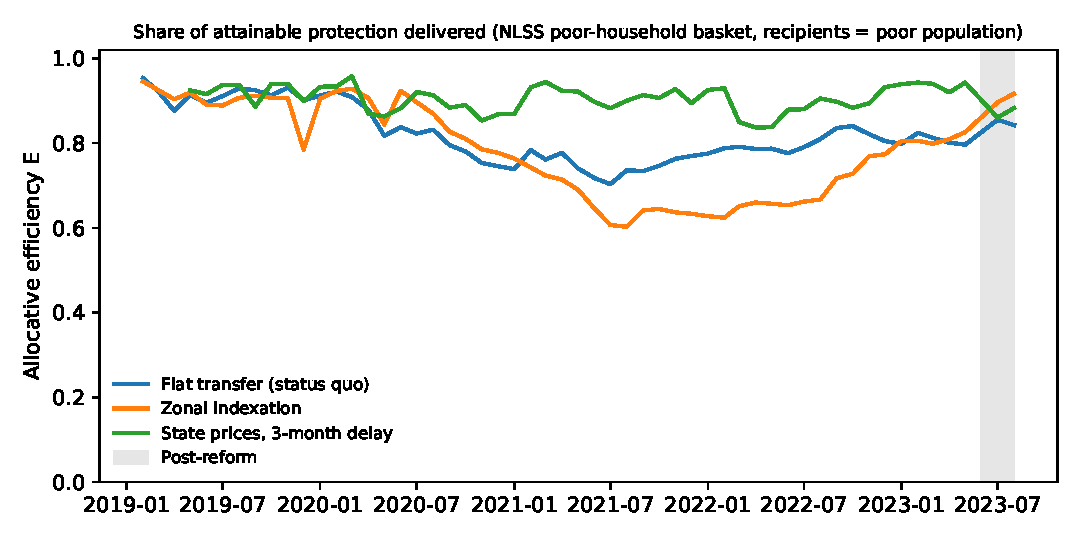
\includegraphics[width=0.92\textwidth]{fig_gate1_nlss.pdf}
\caption{Allocative efficiency $E$ of three simple rules, January 2019 base, NLSS 2018/19 poor-household weights, recipients equal to each state's poor population. Shaded: after the May 2023 reforms (genuine state data to August 2023).}\label{fig:gate1}
\end{figure}

\subsection{Experimental design}\label{sec:design}

All experiments are rolling and use only information available at decision time. In month $t$ the planner sees the published zonal averages for month $t$ and the full state panel up to month $t-1$.

\paragraph{Rules.} We compare (i) a \emph{flat} transfer; (ii) \emph{zonal} indexation, $T\propto D(\bar p^{Z}_t)$; (iii) the \emph{plug-in} rule, $T\propto\hat D_t$, where $\hat D_{st}$ is the need at zonal average prices multiplied by each state's median relative price over the previous 12 months, corrected by the median residual of the previous 12 months; (iv) the robust rule $T^{\mathrm{rob}}$; and (v) the guarantee-constrained rules $T^\kappa$ of \cref{prop:kappa} with $\kappa\in\{0.5,0.8,0.85,0.9,0.95,1\}$, all centred on the plug-in forecast.

\paragraph{Uncertainty sets.} The price polytope uses relative-price bands with 12-month rolling centres and scales, a simultaneous conformal quantile over a 24-month calibration window, and either zonal averages alone (I1) or zonal averages and published state extremes (I2); it is solved by \cref{prop:knapsack}. The need box uses the same windows on the 37 need residuals (\cref{prop:needbox}). Both use adaptive conformal inference with target miss rate $\alpha=0.20$ and step $\gamma=0.02$.

\paragraph{Metrics.} For each month we record the realised efficiency $E(T,p_t)$ of every rule at the true state prices, the guarantee $G_t$, the certified efficiency $\theta(T)$ of every rule (\cref{thm:robust}), and whether the true needs fell inside the box. Bands need 48 months of history, so the need-box evaluation covers January 2021 to August 2023 (31 months) and the price-polytope evaluation January 2020 to August 2023 (43 months).

\paragraph{Robustness.} Every experiment is repeated with national instead of zonal basket weights, with all-household instead of poor-household weights, and without the ``other grains'' group, whose mapping to NBS items is the least certain.

\subsection{Results}\label{sec:results}

\subsubsection{Price polytopes and need boxes}

With 1{,}554 price cells, a simultaneous band that covers all of them in 80\% of months has to be wide. With zonal averages only (I1), the price-polytope guarantee averaged 0.28 and the robust rule realised 0.76, below the flat rule (0.80). Adding the published state extremes (I2) raised the guarantee to 0.61 and realised efficiency to 0.79. The extremes therefore carry much of the information in the published data, but the price-level model is still too cautious to improve on the flat rule. The remaining results use the need box.

\subsubsection{Realised and certified efficiency}

\Cref{tab:frontier} and \cref{fig:frontier} report the results for the need box. The flat rule realised on average 0.784 of attainable protection and zonal indexation 0.689. The plug-in rule realised 0.922, with a minimum of 0.855, and so recovered 64\% of the protection lost by the flat rule using only published aggregates and past state data. Its certificate was low, 0.465 on average. With $\kappa=0.9$ the guarantee-constrained rule realised 0.910, 1.2 points less than the plug-in rule, and its certificate rose to 0.642. With $\kappa=1$ the certificate reached the guarantee $G=0.713$ and realised efficiency fell to 0.871. In every month the realised efficiency of every rule was at least its certificate. The calibrated box contained the true needs in 87\% of months against a target of 80\%; certificates also held in the remaining months because the worst case they bound was not realised.

\begin{table}[t]
\centering
\caption{Realised and certified efficiency, January 2021 to August 2023 (31 months), poor-household zonal weights, need box with adaptive conformal calibration at $\alpha=0.20$. ``Holds'': share of months in which realised efficiency was at least the certificate.}\label{tab:frontier}
\begin{tabular}{lccccc}
\toprule
Rule & \multicolumn{2}{c}{Realised $E$} & \multicolumn{2}{c}{Certified $\theta$} & Holds\\
\cmidrule(lr){2-3}\cmidrule(lr){4-5}
 & mean & min & mean & min & \\
\midrule
Flat & 0.784 & 0.703 & 0.403 & 0.241 & 1.00\\
Zonal & 0.689 & 0.586 & 0.346 & 0.187 & 1.00\\
Plug-in & 0.922 & 0.855 & 0.465 & 0.332 & 1.00\\
$\kappa=0.8$ & 0.917 & 0.847 & 0.570 & 0.534 & 1.00\\
$\kappa=0.85$ & 0.915 & 0.843 & 0.606 & 0.567 & 1.00\\
$\kappa=0.9$ & 0.910 & 0.836 & 0.642 & 0.601 & 1.00\\
$\kappa=0.95$ & 0.901 & 0.819 & 0.677 & 0.634 & 1.00\\
Robust ($\kappa=1$) & 0.871 & 0.779 & 0.713 & 0.667 & 1.00\\
\bottomrule
\end{tabular}
\end{table}

\begin{figure}[t]
\centering
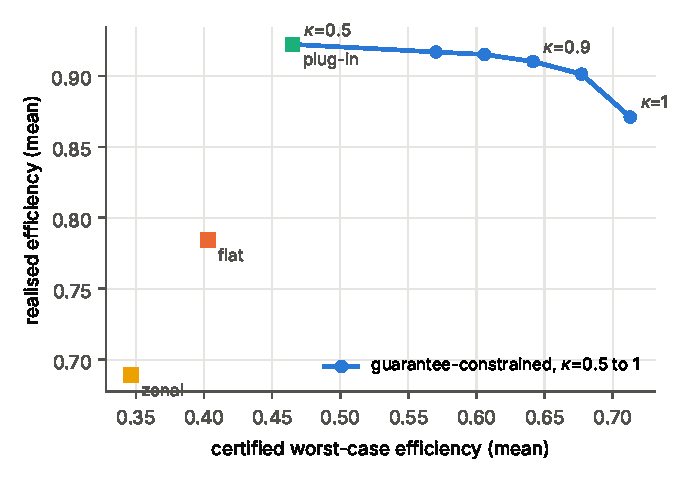
\includegraphics[width=0.62\textwidth]{fig_frontier.pdf}
\caption{Frontier between certified worst-case efficiency and realised efficiency (means over 31 test months). The guarantee-constrained rules of \cref{prop:kappa} dominate the flat and zonal rules on both axes.}\label{fig:frontier}
\end{figure}

\subsubsection{Robustness}

The ranking of the rules is the same under all four weight variants. Realised efficiency of the $\kappa=0.9$ rule ranged from 0.907 to 0.922 and its certificate from 0.639 to 0.677. The flat rule ranged from 0.784 to 0.799 and zonal indexation from 0.678 to 0.692.

\subsubsection{Monitoring}

\Cref{fig:monitoring} shows the mean guarantee over the 13 test months (July 2022 to August 2023) when the monitored states are chosen by \cref{alg:greedy} on the 15 training months. Without delay, monitoring three states raised the guarantee from 0.721 to 0.772, five states to 0.792, ten to 0.837 and fifteen to 0.875. The first states selected were Kano, Sokoto and FCT Abuja, followed by Jigawa, Kaduna, Katsina, Zamfara and Kebbi. Most are populous states with many poor recipients, and FCT is the state whose need is hardest to forecast from zonal averages. For $K\le3$ the greedy selection coincided with the exhaustive optimum. Selection by the guarantee gave a higher guarantee than selection by forecast accuracy at every $K$ (0.772 against 0.760 at $K=3$ and 0.837 against 0.825 at $K=10$), while realised efficiency was similar for both, between 0.92 and 0.93.

With a one-month reporting delay the guarantee stayed between 0.725 and 0.739 for any number of monitored states, and with a three-month delay between 0.726 and 0.752. A delayed report narrows the band of a state much less than a timely one, and because the calibration is simultaneous across states, most of that narrowing is lost. A few states reported promptly therefore raise the guarantee more than many states reported late.

\begin{figure}[t]
\centering
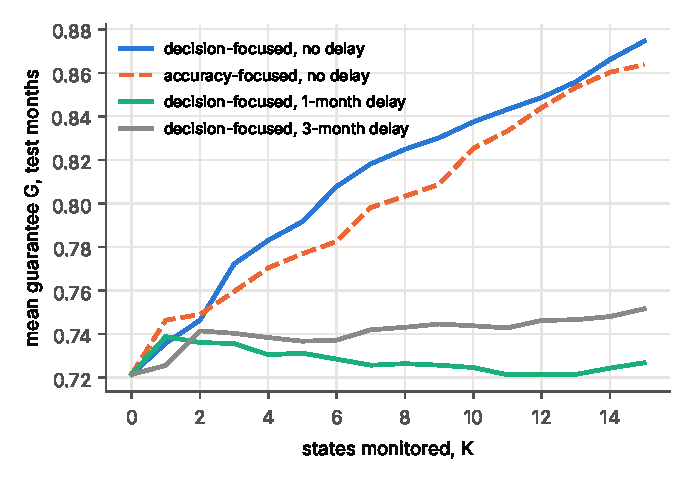
\includegraphics[width=0.62\textwidth]{fig_monitoring.pdf}
\caption{Mean guarantee $G$ on test months against the number of monitored states, by reporting delay and selection criterion.}\label{fig:monitoring}
\end{figure}

\subsubsection{Application to September 2023 to May 2026}

No state food prices were published after August 2023. We forecast needs by \eqref{eq:stale} from August 2023, taking both ends of the zonal growth ratio from the published zonal series, and calibrate the bands by horizon on the full 2017--2023 history. These bands use a longer calibration sample than the 24-month windows of the backtest, so their level should not be compared with \cref{tab:frontier}; the change over the horizon is the quantity of interest. From January 2025 NBS publishes averages for 26 of our 42 items, and needs are computed on these items with weights rescaled to sum to one. \Cref{fig:live} shows the results. The guarantee fell from 0.876 in September 2023 to 0.738 in December 2024 and 0.671 in May 2026. Over the same period the certificate of the $\kappa=0.9$ rule fell from 0.835 to 0.604, that of the flat rule from 0.699 to 0.387 and that of zonal indexation from 0.786 to 0.356. By 2026 the flat rule was certified to deliver only about two fifths of attainable protection, against 60\% for the guarantee-constrained rule.

In May 2026 the $\kappa=0.9$ rule paid FCT Abuja 1.56 times the flat amount, Imo 1.32 times and Ebonyi, Oyo and Cross River about 1.26 times, and it paid Kogi and Plateau 0.83 and 0.80 times. The forecast alone would pay FCT 0.94 times the flat amount. The difference comes from the floor $f_s$ in \eqref{eq:waterfill}. FCT's need relative to its zonal average rose by more than 60\% between January 2019 and mid-2021 and fell back by 2023, so its band at a 33-month horizon is the widest of all states, with a half-width of 0.86 in logs against a median of 0.18. FCT has 2\% of the recipients, so raising its floor costs little of the budget. Monitoring FCT, the third state selected by \cref{alg:greedy}, would narrow its band and lower this floor.

\begin{figure}[t]
\centering
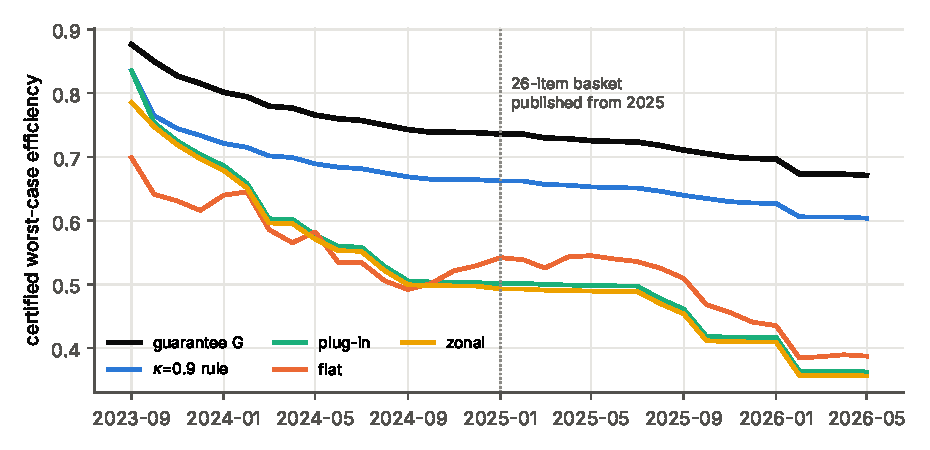
\includegraphics[width=0.9\textwidth]{fig_live.pdf}
\caption{Guarantee and certified efficiency of four rules, September 2023 to May 2026, when only national and zonal averages and state extremes are published. Bands widen with months since the last state data (August 2023).}\label{fig:live}
\end{figure}

% =====================================================================
\section{Discussion and policy implications}\label{sec:discussion}

\subsection{Implications for social-protection programmes}

Over 2021 to 2023 a flat national transfer delivered 78\% of the protection that the same budget could have delivered, and indexation to zonal averages delivered 69\%. The guarantee-constrained rule needs no data beyond the published zonal averages and the state history to August 2023. Each state receives a floor proportional to its worst-case need share, and the rest of the budget is distributed in proportion to forecast need. The parameter $\kappa$ sets the balance between the two. With $\kappa=0.9$ the rule loses about one point of realised efficiency relative to the plug-in rule and raises the certified worst case by about 18 points. Each payment can be traced to a published average, a historical premium and a calibrated band, and the part of a payment that comes from the floor can be reported separately. A payment well above the forecast, as for FCT, identifies a state whose need is poorly known and is a reason to monitor that state.

\subsection{Implications for statistical agencies}

The guarantee gives a value to each source of price information. The published highest- and lowest-priced states more than doubled the guarantee of the price-level model. Prompt publication of a few populous northern states (Kano, Sokoto, Jigawa and Kaduna) together with FCT Abuja would raise the guarantee more than delayed publication of many states. Without state tables since September 2023, the certified protection of every rule has declined, and by 2026 the flat rule is certified at 39\%.

% =====================================================================
\section{Conclusions, limitations and future research}\label{sec:conclusion}

This paper studied the allocation of a fixed transfer budget across regions when local food prices are known only through aggregates, extremes and delayed data. For (Q1), the robust allocation pays each region in proportion to its largest possible need share, and the guarantee-constrained rules of \cref{prop:kappa} keep most of the accuracy of a good forecast while bounding the loss when the forecast fails. For (Q2), need boxes calibrated by adaptive conformal prediction gave certificates that held in every test month. In the backtest, with state data one month old, the guarantee averaged 0.71; after August 2023 it fell as the state data aged, to 0.67 by May 2026. For (Q3), greedy selection by the guarantee matched the exhaustive optimum for up to three states and outperformed selection by forecast accuracy, and reporting delay limited the value of monitoring more than the number of monitored states.

The study has several limitations. The priced basket covers 88\% of the food spending of poor households, and the number of recipients in each state is approximated by its poor population in 2019. The evaluation period contains one large shock, so the coverage of the bands across regimes relies on the adaptive method. The bands for stale data are calibrated on overlapping historical windows, and at long horizons they rest on few independent episodes. The backtest computes zonal averages from state prices, whereas the published zonal averages for April to August 2023 differ from these item by item. We do not model behavioural or price responses to the transfers.

Future work could treat prices and recipient numbers as jointly uncertain, allocate at the level of local government areas using satellite or market data as side information, and select items as well as states for monitoring with explicit survey costs.

\section*{Data and code availability}
Code and derived data are available at \url{https://github.com/Manirmaths/robust-food-indexed-transfers}\todo{archive on Zenodo and add DOI}. Food prices are from the NBS Selected Food Price Watch \citep{nbs2026econs}. NLSS 2018/19 microdata \citep{nlss2019} are available from the World Bank Microdata Library under its terms of use and are not redistributed.

\IfFileExists{elsarticle-num.bst}{\bibliographystyle{elsarticle-num}}{\bibliographystyle{plainnat}}
\bibliography{refs}

\end{document}
